\documentclass[UTF8]{ctexart}
\usepackage{hyperref}
\usepackage{abstract}
\usepackage[margin=1in]{geometry}
\usepackage{graphicx}
\usepackage{gensymb}
\usepackage{amsmath}
\usepackage{float}
\usepackage{ctex,amsmath,amssymb,bm,indentfirst,hyperref,graphicx}
\usepackage{multirow}
\begin{document}

\title{第二次仿真作业}
\author{2019012137  工物90  张鸿琳}
\maketitle

\tableofcontents
\newpage

\section{题目一:占空比可调的脉冲序列发生器}
\subsection{电路原理图及分析}
电路原理图如下:
\begin{figure}[H]
\centering
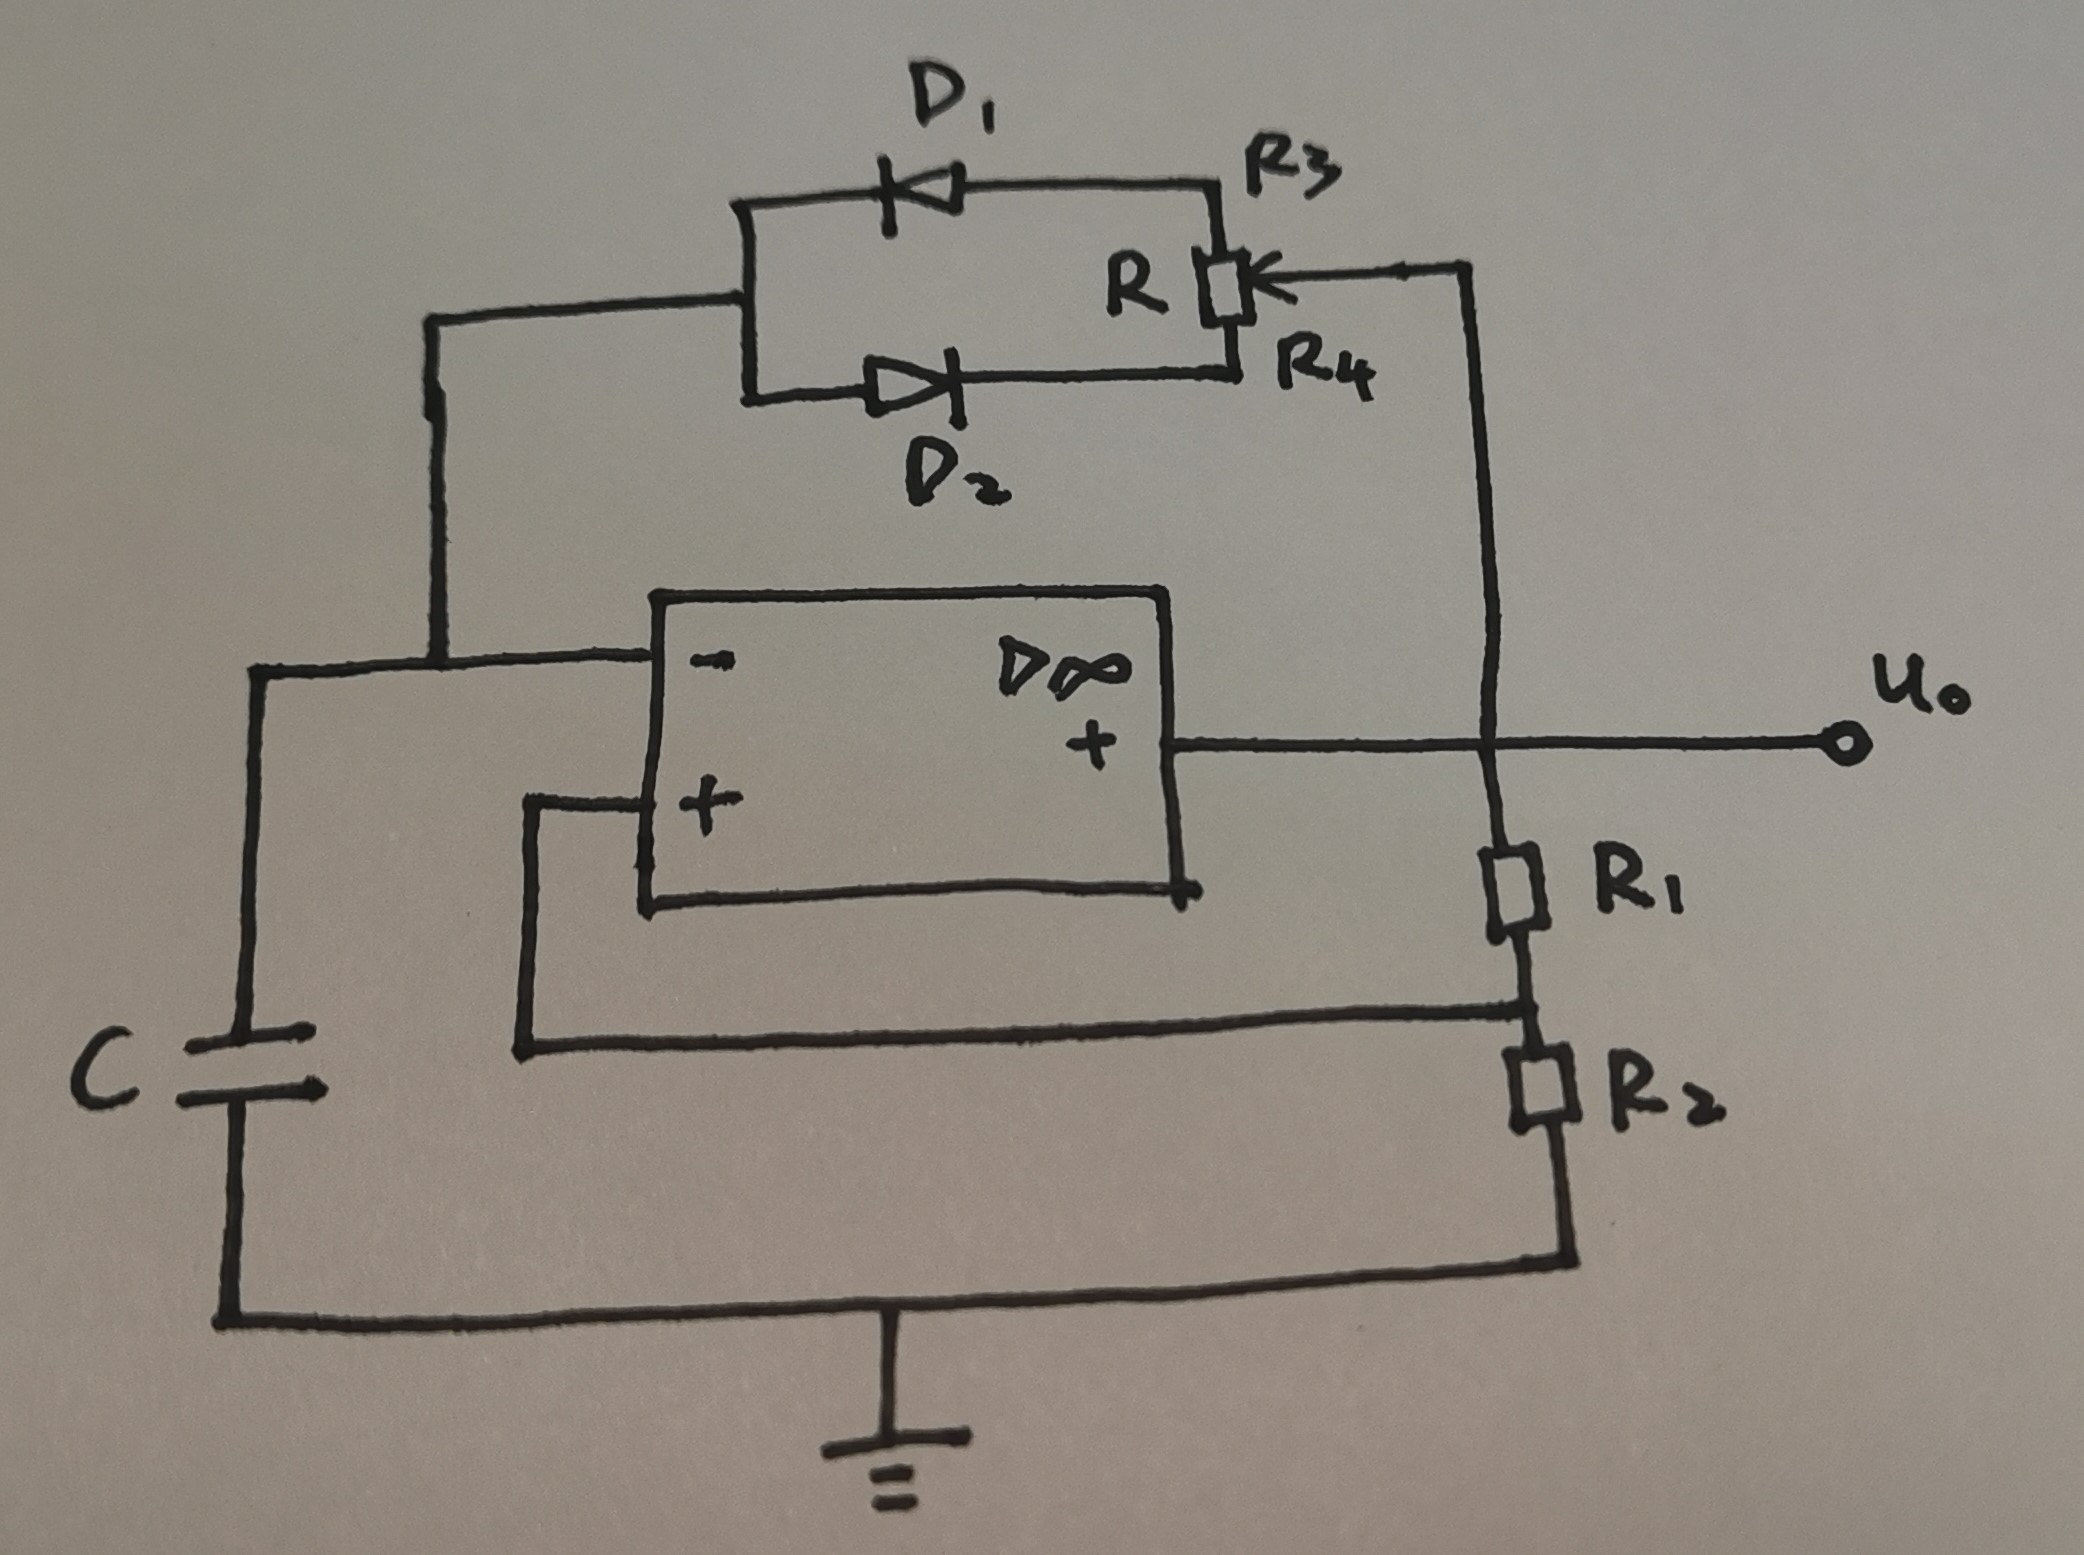
\includegraphics[width=0.95\textwidth]{A.jpg}
\caption{占空比可调的脉冲序列发生器的手绘电路原理图}
\end{figure}

图中$R_1$=$R_2$,由于微小扰动,$u_0$达到饱和电压,不妨设为$U$,则运放的同相输入电压为$\frac{U}{2}$,电容器初始电压$u_C$为零,故而初始时,电流通过滑动变阻器的上半部分$R_3$,以及二极管$D_1$,给电容器$C$充电,直到电容器电压达到$\frac{U}{2}$时,$u_0$瞬间达到反向饱和电压$U$,同相输入电压变为$-\frac{U}{2}$,此时电容器开始放电并反向充电,电流通过二极管$D_2$以及滑动变阻器的下半部分$R_4$,直到电压达到$-\frac{U}{2}$,此后达到稳定电容器电压在$\frac{U}{2}$与$-\frac{U}{2}$之间周期性变化,由此生成周期性方波状的$u_0$。

由上面的分析,经过计算,可知电容器电压由$-\frac{U}{2}$开始随时间变化为$u_C=-\frac{3}{2}Ue^{-\frac{t}{R_3C}}+U$,则变化到$\frac{U}{2}$所需时间为$CR_3\ln3$。同理可得电容器电压由$\frac{U}{2}$变化到$-\frac{U}{2}$所需时间为$CR_4\ln3$,故而可知,生成的方波脉冲的周期为$C(R_3+R_4)\ln3=CR\ln3$,其中$R$为滑动变阻器总阻值,其中$CR_3\ln3$的时间,输出电压为$U$,$CR_4\ln3$的时间,输出电压为$-U$,所以占空比为$\frac{R_3}{R_3+R_4}=\frac{R_3}{R}$,故而可以通过调节滑动变阻器,改变$R_3$的大小来调节占空比,同时不改变周期。

\subsection{仿真电路图}
占空比可调的脉冲序列发生器的仿真电路图如下:
\begin{figure}[H]
\centering

\includegraphics[width=0.95\textwidth]{B.png}
\caption{占空比可调的脉冲序列发生器的仿真电路原理图}
\end{figure}

\subsection{示波器波形图}
占空比为$20\%$时,脉冲序列波形和对应的电容电压波形如下(脉冲序列波形为方波):
\begin{figure}[H]
\centering
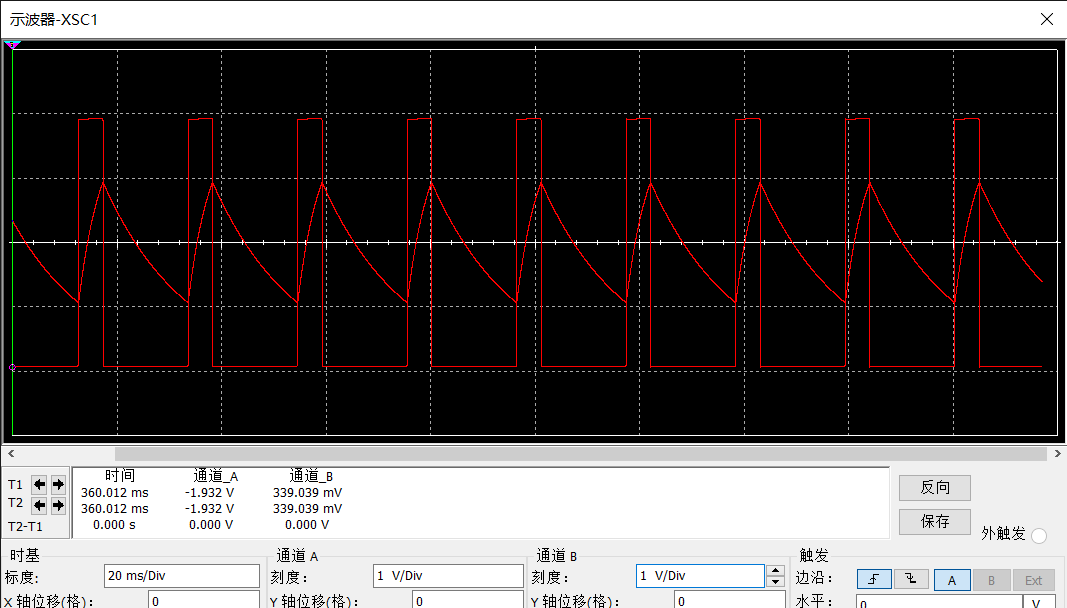
\includegraphics[width=0.95\textwidth]{CC.png}
\caption{占空比为$20\%$时,脉冲序列波形和对应的电容电压波形}
\end{figure}

占空比为$70\%$时,脉冲序列波形和对应的电容电压波形如下(脉冲序列波形为方波):
\begin{figure}[H]
\centering
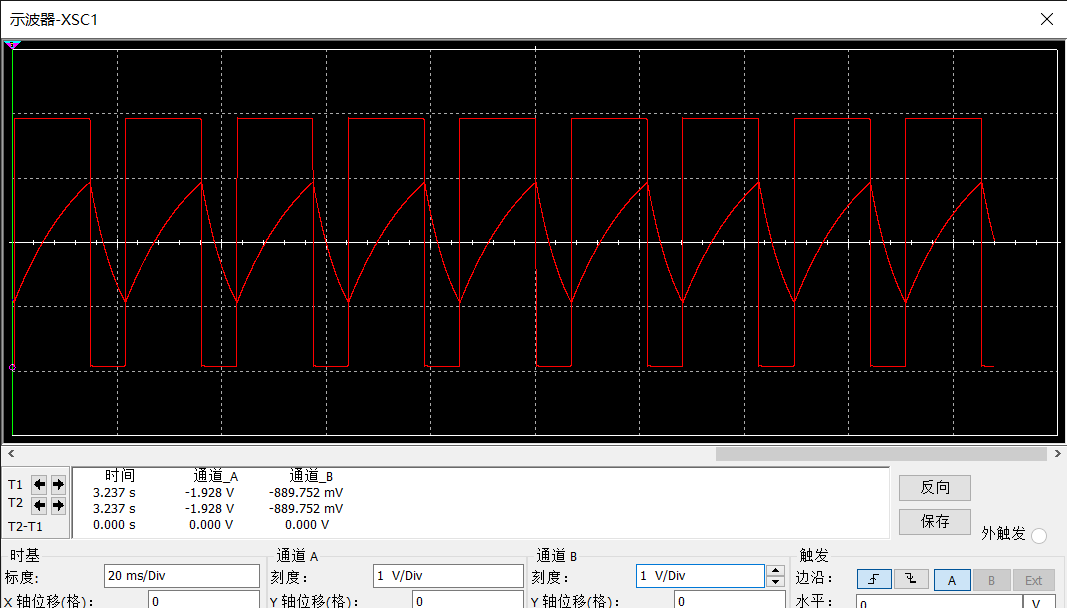
\includegraphics[width=0.95\textwidth]{DD.png}
\caption{占空比为$70\%$时,脉冲序列波形和对应的电容电压波形}
\end{figure}

\section{三角波发生器}
\subsection{电路原理图及分析}
电路原理图如下:
\begin{figure}[H]
\centering
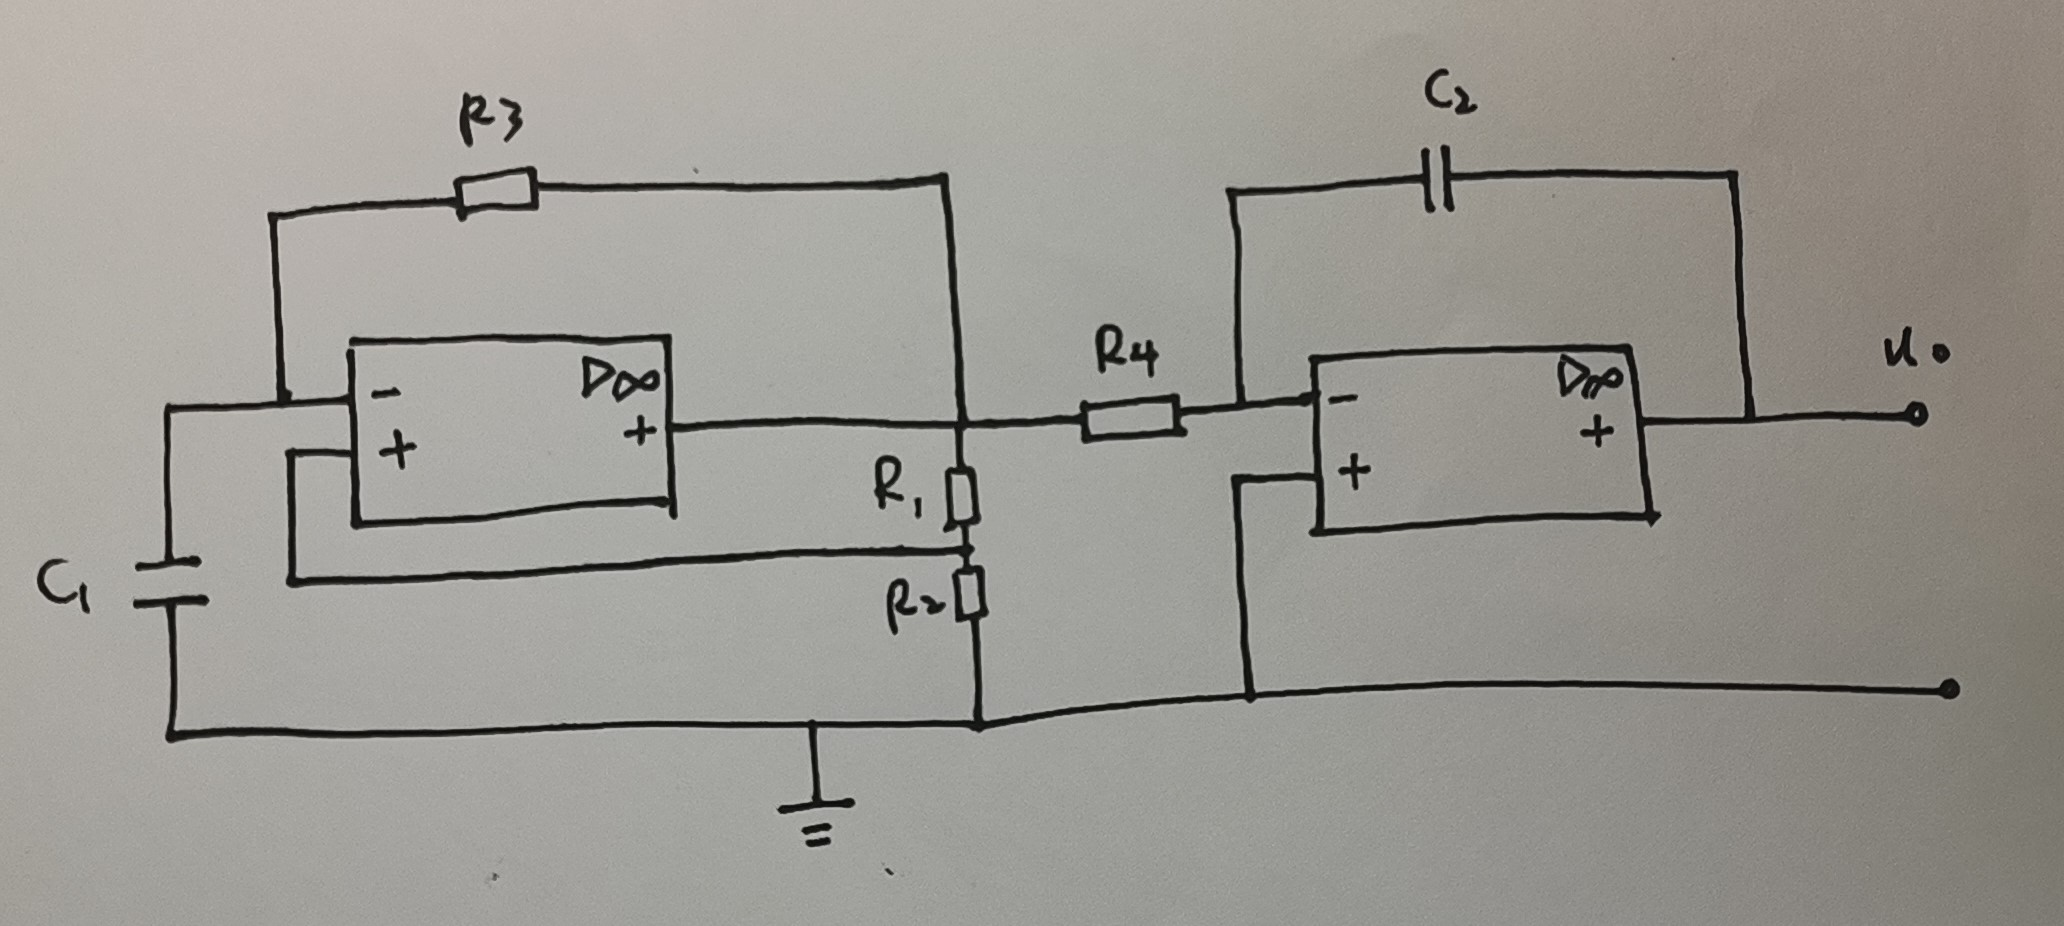
\includegraphics[width=0.95\textwidth]{G.jpg}
\caption{三角波发生器的手绘电路原理图}
\end{figure}

假设$R_4$左侧电势为定值$U$,则输出电压$u_0$的变化应满足
\begin{equation}
\frac{U}{R_4}=-C_2\frac{du_0}{dt}
\end{equation}

解得(设$u_0$初值为0)$u_0$=$-\frac{U}{R_4C_2}t$,为过零点的斜率为$-\frac{U}{R_4C_2}$的直线,那么如果输入为周期性跳变为$U$和$-U$,那么输出就为三角波,所以在$R_4$左侧加上一个脉冲序列发生器即可输出三角波。

\subsection{仿真电路图}

三角波发生器的仿真电路图如下:
\begin{figure}[H]
\centering
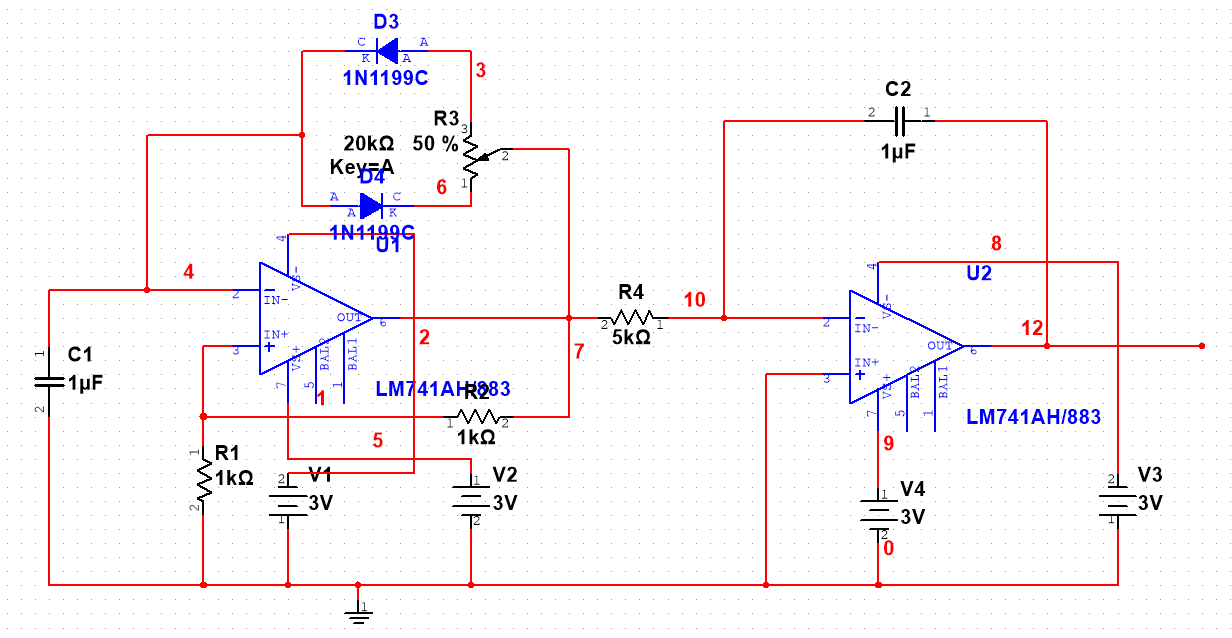
\includegraphics[width=0.95\textwidth]{E.png}
\caption{三角波发生器的仿真电路原理图}
\end{figure}
\subsection{示波器波形图}
脉冲序列和三角波的波形在示波器上的显示如下:
\begin{figure}[H]
\centering
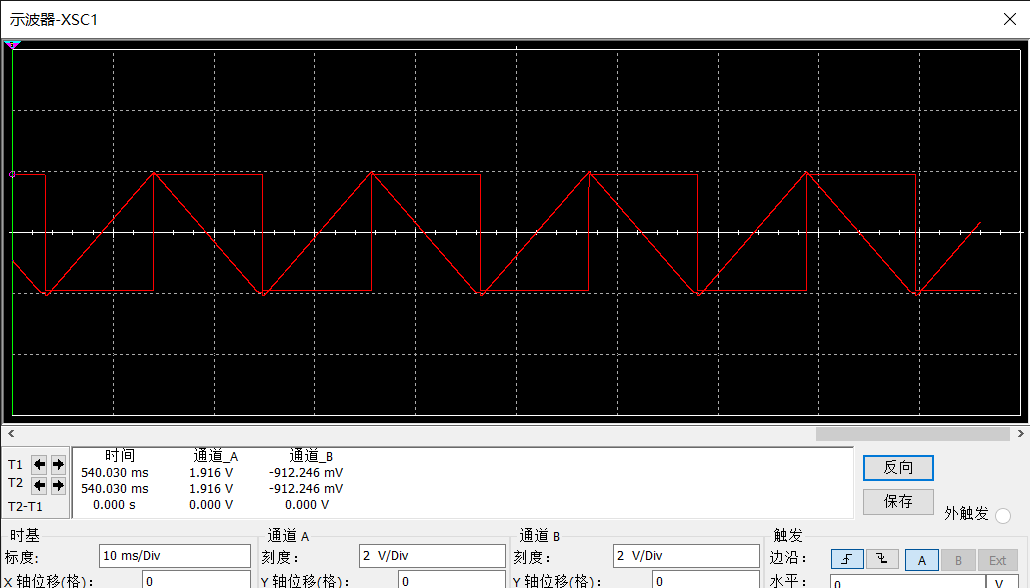
\includegraphics[width=0.95\textwidth]{F.png}
\caption{三角波发生器的示波器波形}
\end{figure}


\begin{thebibliography}{123456} 
\bibitem{ref1} 无
\end{thebibliography}


\end{document}
